% \clearpage

\section{Rare Z and Higgs decays to quarkonia}
\label{section_rare_deays}

The rare decays of the Higgs boson~\cite{higgs_discovery_atlas,higgs_discovery_cms} to a quarkonium state and a photon provide a unique sensitivity to the magnitude of the Yukawa couplings of the Higgs boson to quarks~\cite{PhysRevD.88.053003, PhysRevD.90.113010,PhysRevLett.114.191803}. These couplings are difficult to access on hadronic collisions through direct decay of Higgs in quark-antiquark, due to the immense background from QCD~\cite{PhysRevD.89.033014}. 

Among the channels available to explore Yukawa's couplings of light quarks~\cite{PhysRevD.90.113010,PhysRevLett.114.191803} the prominent candidates are those with heavy-quarkonia. The rare modes of decay of the \Z boson have attracted attention focused on establishing its sensitivity to New Physics \cite{PEREZ}, being an alternative environment to investigate the Yukawa couplings of the Higgs boson.

% Several estimates of the branching ratio of the Standard Model for the decay of the vector bosons in simple vector meson + photon are available with the latest branching ratio value of the order of $10^{-8}$ and compatible with results published by the ATLAS collaboration~\cite{atlas_results_2016_data}. Thus, the objective of this physics analysis is to explore exclusive rare decays of vector bosons in the CMS experiment using the data taken during 2016.

Also, the exclusive rare decays of vector bosons (\Z, W) provide a favorable environment for testing the factorization of QCD, thus allowing an approach in a context where the power of corrections are definitely under control. The main focus of this kind of analysis are the hadronic radioactive decays, $Z\rightarrow M \gamma$, where M can be a pseudoscalar or a vector meson ($J/ \Psi, \phi, \Upsilon_{n}$). 

They offer the perfect way to explore some of the leading order properties of the light-cone distribution amplitudes (LCDAs)~\cite{Grossman2015} of several mesons, but they present a difficulty, considering that in the LHC energy scale the branching ratio of these processes is very small. There are theoretical predictions~\cite{PhysRevD.97.016009,PhysRevD.96.116014} that point out a branching ratio for several decay channels in the Standard Model, as shown in the Table \ref{fig:XsecTable}.

\begin{table}[htp]
  \begin{center}
    \caption{Summary of branching ratios for $H/Z \rightarrow \Upsilon(1S,2S,3S)+\gamma  \rightarrow \mu^{+} \mu^{-} +\gamma$ analysis. The effective cross-section will be discussed in section \ref{sec:datasets}.}
    %\resizebox{.5\width}{!}{\begin{tabular}{l|llll}
\multicolumn{4}{c}{95\% C.L. Upper Limit} \\
\hline
\hline
& \multicolumn{3}{c}{$\mathcal{B}(Z \rightarrow \Upsilon\gamma)$ $[\times10^{-6}]$}      \\
\cline{2-4}
&  $\Upsilon(1S)$ & $\Upsilon(2S)$ & $\Upsilon(3S)$  \\
\hline
Expected     & $6.4^{+3.1}_{-2.0}$ &  $8.3^{+4.0}_{-2.5}$  & $8.0^{+3.9}_{-2.4}$            \\
Observed     & 9.0 &  12.3  & 11.4      \\
\hline
SM Prediction $[\times10^{-8}]$ & 4.8  &  2.4  & 1.9      \\
\hline
\hline
& \multicolumn{3}{c}{$\mathcal{B}(H \rightarrow \Upsilon\gamma)$ $[\times10^{-4}]$}       \\
\cline{2-4}
&  $\Upsilon(1S)$ & $\Upsilon(2S)$ & $\Upsilon(3S)$ &   \\
\hline
Expected     & $12.5^{+6.1}_{-3.9}$ &  $14.6^{+7.1}_{-4.5}$  & $13.6^{+6.6}_{-4.2}$        \\
Observed     & 11.5 &  13.6  & 12.7     \\
\hline
SM Prediction $[\times10^{-9}]$ & 5.2  &  1.4  & 0.9      \\
\hline
\hline
\end{tabular}

}
    %%\begin{table}[htp]
%%\begin{center}
%\begin{tabular}{|c|l|l|}
%\hline
%Description of the Physics Processes  : & Cross Section ( $\sigma$ in pb) & Branching Ratio (BR$_{SM}$): \\ \hline
%H$\rightarrow  \Upsilon(1S) +\gamma$ & 7.1996$\times 10^{-9}$ &5.22$\times 10^{-9}$ \\ \hline
%H$\rightarrow  \Upsilon(2S) +\gamma$ & 1.5242$\times 10^{-9}$ &1.42$\times 10^{-9}$ \\ \hline
%H$\rightarrow  \Upsilon(3S) +\gamma$ & 1.1033$\times 10^{-9}$ &9.10$\times 10^{-10}$ \\ \hline \hline
%%Z$\rightarrow J/ \psi +\gamma$ & 9.9123$\times 10^{-6}$ & 2.99$\times 10^{-6}$ \\ \hline
%Z$\rightarrow  \Upsilon(1S) +\gamma$ & 6.7965$\times 10^{-5}$ &4.88$\times 10^{-8}$ \\ \hline
%Z$\rightarrow  \Upsilon(2S) +\gamma$ & 2.6887$\times 10^{-5}$ &2.44$\times 10^{-8}$ \\ \hline
%Z$\rightarrow  \Upsilon(3S) +\gamma$ & 2.3400$\times 10^{-5}$ &1.88$\times 10^{-8}$ \\ \hline \hline
%H$\rightarrow \gamma\gamma^{*}$ Dalitz Decay & 1.8614$\times 10^{-3}$ & 3.83$\times 10^{-5}$ \\ \hline
%Z$\rightarrow  \mu\mu\gamma_{FSR}$ & 7.9260$\times 10^{-2}$& --- \\ \hline
%
%\end{tabular}
%%\caption{Summary of data samples used for $H/Z \rightarrow \Upsilon(1S,2S,3S)+\gamma$ analysis }
%%\label{Tablebkg}
%%\end{center}
%%\end{table}
%% Ref latex: https://tex.stackexchange.com/questions/112343/beautiful-table-samples
%



%\begin{table}[htp]
%\begin{center}
\begin{tabular}{c|c}
\hline
Physics Processes & Branching Ratio (BR$_{SM}$): \\ \hline
H$\rightarrow  \Upsilon(1S) +\gamma$ & 5.22$\times 10^{-9}$ \\ \hline
H$\rightarrow  \Upsilon(2S) +\gamma$ & 1.42$\times 10^{-9}$ \\ \hline
H$\rightarrow  \Upsilon(3S) +\gamma$ & 9.10$\times 10^{-10}$ \\ \hline \hline
Z$\rightarrow  \Upsilon(1S) +\gamma$ & 4.88$\times 10^{-8}$ \\ \hline
Z$\rightarrow  \Upsilon(2S) +\gamma$ & 2.44$\times 10^{-8}$ \\ \hline
Z$\rightarrow  \Upsilon(3S) +\gamma$ & 1.88$\times 10^{-8}$ \\ \hline 
%H$\rightarrow \gamma\gamma^{*}$ Dalitz Decay & 1.8614$\times 10^{-3}$ & 3.83$\times 10^{-5}$ \\ \hline
%Z$\rightarrow  \mu\mu\gamma_{FSR}$ & 7.9260$\times 10^{-2}$& --- \\ \hline

\end{tabular}
%\caption{Summary of data samples used for $H/Z \rightarrow \Upsilon(1S,2S,3S)+\gamma$ analysis }
%\label{Tablebkg}
%\end{center}
%\end{table}
% Ref latex: https://tex.stackexchange.com/questions/112343/beautiful-table-samples


    %\caption{Summary of cross section and branching ratio for $H/Z \rightarrow \Upsilon(1S,2S,3S)+\gamma  \rightarrow \mu^{+} \mu^{-} +\gamma$ analysis. Assuming that of $\sigma (pp\rightarrow$ H) is 55.614 $pb^{-1}$ and  $\sigma (pp\rightarrow Z \rightarrow \mu\mu$ ) is 57094.5 $pb^{-1}$ with the phase space selection in invariant mass of the dimuon system of $m_{\mu\mu} > 50 GeV$ (Missing References). }
    \label{fig:XsecTable}
  \end{center}
\end{table}





%Table
% https://docs.google.com/spreadsheets/d/1zP8P9kp-yFrkMu9bGt4fpIirKAKYlH-w2em_kVkYYKw/edit?usp=sharing
%Pag2

Recent studies on exclusive Higgs boson decays \cite{ISIDORI2014131,PhysRevLett.114.101802,GAO2014366} in final states containing a vector meson and a photon have caused interest in these physics topics. It was proposed to use these decays as a possible way to explore non-standard Yukawa couplings of the Higgs boson. Such measures are quite challenging in the LHC environment. The observation of hadronic decays of vector bosons could provide a new frontier for the nature of heavy quarkonia production in hadronic collisions.

Along the same lines, the simple exploration of rare SM decays, even in scenarios where anomalous couplings are, in principle, ruled out by direct measurements~\cite{cms_h_to_bb_PhysRevLett.121.121801}, as in the case of this analysis ($H \rightarrow \Upsilon(nS) + \gamma$), are still important as a stress test of the SM and as reference for future measurements. Specially the later one, when you consider that the small predicted cross sections from Table~\ref{fig:XsecTable}, most probably, would imply that an observation of this decay would be unlikely even in the HL-LHC~\cite{hl_lhc}.

This measurement is sensitive to the direct and indirect production (Figure~\ref{direct_indirect}). The \textit{direct} process consists in the decay of boson (Higgs or Z) to a quark anti-quark pair, in which, one of the quarks radiates a photon and the pair hadronizes to a meson (a $\Upsilon(nS)$, for this study), while in \textit{indirect} process, the decay happens to a $\gamma \gamma^{*}(Z)$, with the subsequent decay of the $\gamma^{*}(Z)$ to a quark anti-quark that hadronizes. 


% direct and indirect decays
\begin{figure}[htbp]
  \centering
  \begin{subfigure}[htbp]{0.4\textwidth}
    \centering
    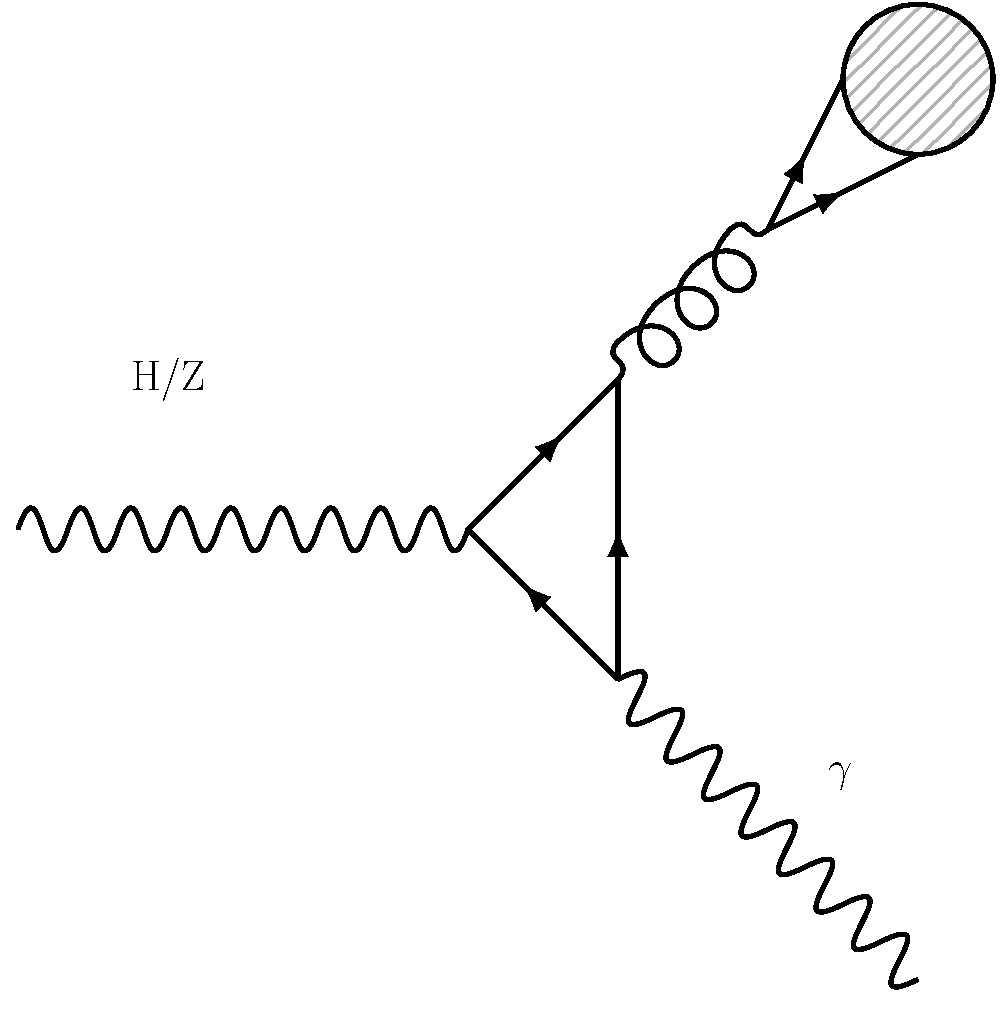
\includegraphics[width=\textwidth]{figures_and_tables/theory/diagrams/indirect}
    \caption{Indirect decay.}
    \label{indirect}
  \end{subfigure}
  \hfill
  \begin{subfigure}[htbp]{0.4\textwidth}
    \centering
    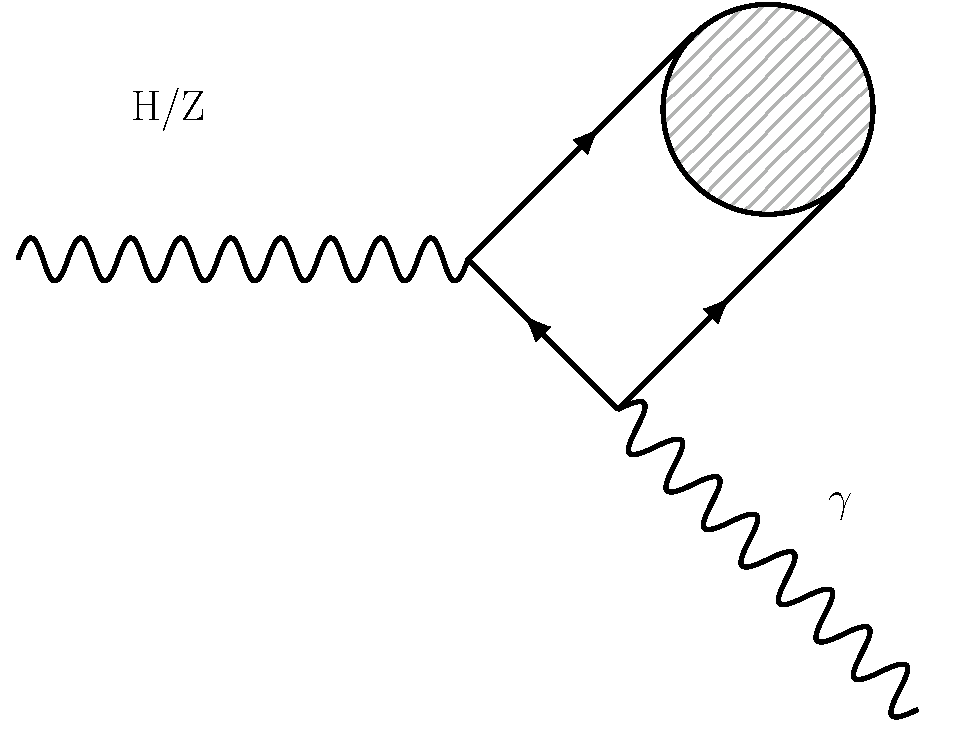
\includegraphics[width=\textwidth]{figures_and_tables/theory/diagrams/direct}
    \caption{Direct decay.}
    \label{direct}
  \end{subfigure}
  \caption{Example of leading order diagrams for the indirect and direct production mechanisms. The dashed blob should be understood as the $\Upsilon(nS)$, where $n=\text{1, 2, 3}$. In the indirect diagram, the majority of the contribution comes from a top loop.}
  \label{direct_indirect}
\end{figure}


Clearly, only the direct process is sensible to the Yukawa coupling of the boson with the quarks, but, since both processes are indistinguishable in their final state, the indirect process needs to be taken into account. In this study, a dimuon final state is used to tag the $\Upsilon(nS)$.

Even though there is different theoretical predictions for the cross section of this process and its twin brother ($H \rightarrow \text{J/}\Psi + \gamma$), each one taking into account different levels of complexity, the 2013 paper~\cite{PhysRevD.88.053003}, from G. Bodwin, F. Petriello, S. Stoynev and M. Velasco, summarizes very well and in a simpler manner, the most relevant phenomenological results on these decays. For the decay to $J/\Psi + \gamma$, the quantum interference with the indirect amplitude, enhances the directed production, leading to a larger, and potentially observable, cross section. This is not true for the $\Upsilon(nS) + \gamma$ decay, since the interference is destructive, diminishing the cross sections. 

Another interesting aspect of this study is that, for both $Hc\bar{c}$ and $Hb\bar{b}$ direct coupling measurements are not sensible to the sign of the Yukawa coupling, while the presence of the indirect process in the $H \rightarrow M + \gamma$ ($M$ standing for J/$Psi$ or $\Upsilon(nS)$) decays resolve this ambiguity.

Finally, since the $\Upsilon(nS) + \gamma$ decay has a much smaller cross section, because of the destructive quantum interference between direct and indirect production mechanisms, a small deviation in the $Hb\bar{b}$ Yukawa coupling, can lead a large increase in the expected branching ratio, making this channel sensible any non-Standard Model process that might interfere in this final state. This becomes clear when we look to Figure~\ref{hbb_coup}.

\begin{figure}[!htbp]
  \begin{center}
    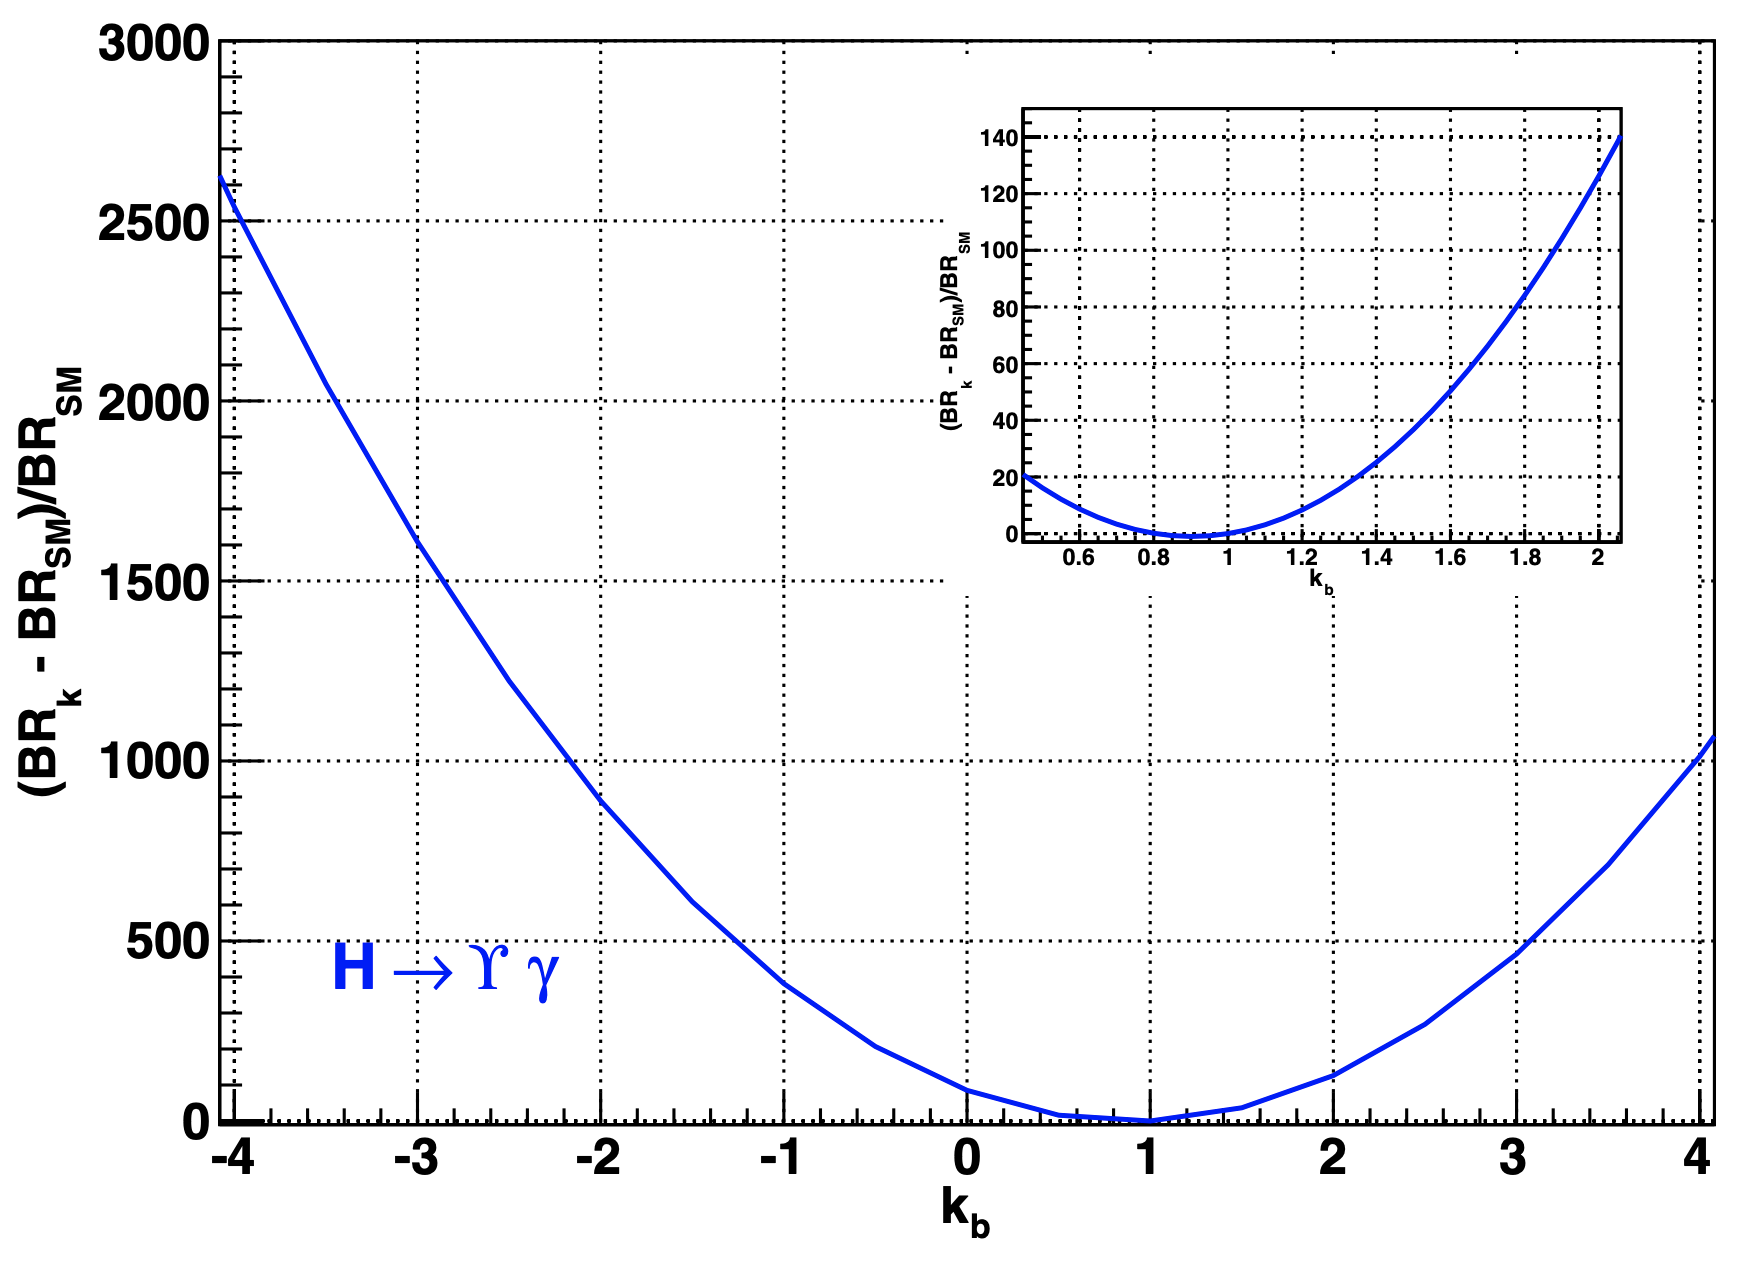
\includegraphics[width=0.6\textwidth ]{figures_and_tables/theory/hbb_coup.png}
  \end{center}\vspace*{-.5cm}
  \caption{Expected relative variation of the branching ratio for the $H \rightarrow \Upsilon(nS) + \gamma$ to $k_b$, where $k_b = g(Hb\bar{b})/g(Hb\bar{b})_{SM}$ is the ratio for the observed and expected Yukawa coupling of $Hb\bar{b}$. Source:~\cite{PhysRevD.88.053003}}
  \label{hbb_coup}
\end{figure}


\section{Recent results}

The ATLAS experiment~\cite{atlas_collaboration_2008} already have two results on this decays~\cite{atlas_paper:PhysRevLett.114.121801, atlas_paper_2018:2018txb}. The first one corresponds to data taken from 2015, while the latter one, corresponds to data from 2016 (the same data taking period to which this study refers).

To what concerns the most updated result, the study corresponded to 36.1 $fb^{-1}$ at $\sqrt{s} = 13$ TeV and no significant excess was found by the experiment. Upper limits for the decay were obtained, assuming the Standard Model branching fractions predictions, at 95\% confidence level, according to Table~\ref{tab:atlas_results_2018}.


\begin{table}[htp]
  \begin{center}
    
    \caption{Observed upper limits, by the ATLAS experiment~\cite{atlas_paper:PhysRevLett.114.121801, atlas_paper_2018:2018txb}, on the branching fractions for the Higgs and Z decays (last result). Detailed comparisons with the results obtained in this study will be presented in Section~\ref{chaper_results}.}
    \begin{tabular}{cc}
      \hline
      Decay & $\mathcal{B}F$ at 95\% \CL \\ \hline
      H$\rightarrow  J/\Psi +\gamma$ & < 4.5$\times 10^{-4}$ \\ 
      H$\rightarrow  \Psi(2S) +\gamma$ & < 2.0$\times 10^{-3}$ \\ 
      H$\rightarrow  \Upsilon(1S) +\gamma$ & < 4.9$\times 10^{-4}$ \\ 
      H$\rightarrow  \Upsilon(2S) +\gamma$ & < 5.9$\times 10^{-4}$ \\ 
      H$\rightarrow  \Upsilon(3S) +\gamma$ & < 5.7$\times 10^{-4}$ \\          
      \hline \hline
      Z$\rightarrow  J/\Psi +\gamma$ & < 2.3$\times 10^{-6}$ \\ 
      Z$\rightarrow  \Psi(2S) +\gamma$ & < 4.5$\times 10^{-6}$ \\ 
      Z$\rightarrow  \Upsilon(1S) +\gamma$ & < 2.8$\times 10^{-6}$ \\ 
      Z$\rightarrow  \Upsilon(2S) +\gamma$ & < 1.7$\times 10^{-6}$ \\ 
      Z$\rightarrow  \Upsilon(3S) +\gamma$ & < 4.8$\times 10^{-6}$ \\        
    \end{tabular}
    \label{tab:atlas_results_2018}
  \end{center}
\end{table}

It is worth it to mention that the ATLAS papers present a broader analysis, including the decays to $J/\Psi +\gamma$ and $\Psi(2S) +\gamma$.


CMS~\cite{cms_paper} also has a result on $J/\Psi +\gamma$ and $\Psi(2S) +\gamma$ decay channel, of the Higgs and Z boson~\cite{papper_jpsi}. The observed upper limits on the branching fraction for these decays are presented in T\ref{tab:cms_jpsi_results}.

\begin{table}[htp]
  \begin{center}
    
    
    \caption{Observed upper limits, by CMS, on the branching fractions for the Higgs and Z decays. The number are compatible with the ones obtained by ATLAS. The results presented for different polarization scenarios of the $J/\Psi$.}
    \begin{tabular}{ ccccc }
      Channel & Polarization  & $\mathcal{B}F$ at 95\% \CL\\
      \hline
      & Unpolarized & $< 1.4\ten{-6}$  \\
      Z$\rightarrow  J/\Psi +\gamma$ & Transverse & $< 1.5\ten{-6}$  \\
      & Longitudinal & $< 1.2\ten{-6}$  \\
      \hline \hline
      H$\rightarrow  J/\Psi +\gamma$ & Transverse & $< 7.6\ten{-4}$  \\
    \end{tabular}
    
    \label{tab:cms_jpsi_results}
  \end{center}
\end{table}

No result on the Z and Higgs decays to $\Upsilon(nS) +\gamma$ have been published by CMS, yet.

The results presented here are a subset of a broader topic related to the rare decays of Standard Model (SM) boson, involving quarkonia. Sticking only to CMS results, we can cite:

\begin{itemize}
  \item Search for Higgs and Z boson decays to $\mathrm{J}/\Psi$ or $\Upsilon$ pairs in proton-proton collisions at $\sqrt{s} = $ 13 TeV~\cite{Sirunyan:2676242}.
  \item Observation of the $\mathrm{Z} \to \Psi \ell^{+}\ell^{-}$ decay in pp collisions at $\sqrt{s} = $ 13 TeV~\cite{Sirunyan:2623687}. This one specifically, is the first observation a such decay, involving a Z boson.
  \item Search for decays of the 125 GeV Higgs boson into a Z boson and a $\rho$ or $\phi$ meson~\cite{cms_higgs_rho_phi}.
\end{itemize}

In this study, we consider the nominal values of mass for the Higgs, Z and the $Y(\text{1S, 2S, 3S})$, as in~\cite{pdg_2020} are considered.

